\definecolor{mDarkTeal}{HTML}{23373b}

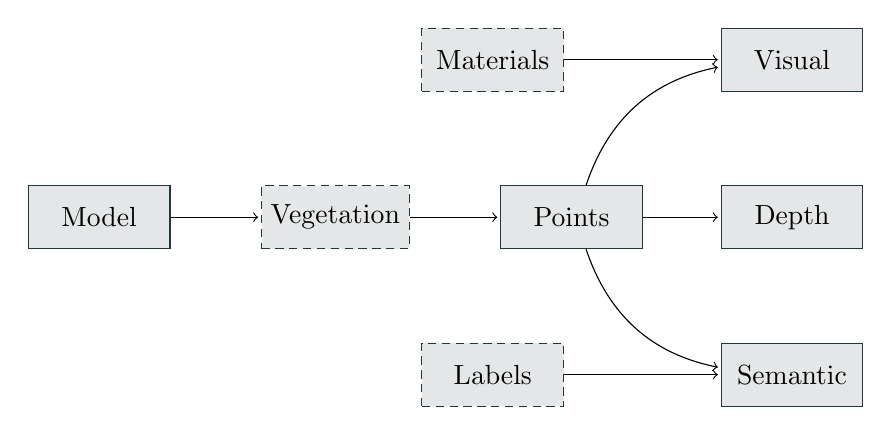
\begin{tikzpicture}
  [var/.style={circle},
  lab/.style={rectangle,draw=mDarkTeal,fill=black!2!white!90!mDarkTeal,
    minimum height=0.8cm,minimum width=1.8cm},
  olab/.style={lab,densely dashed},
  pre/.style={<-,shorten <=1pt,draw},
  post/.style={->,shorten >=1pt,draw}]

%  \clip (1.5,-2.5) rectangle (14.5,4.5);

  \node[lab] (mod) at (0,0) {Model};

  \node[olab] (veg) at (3,0) {Vegetation}
  edge[pre] (mod);

  \node[lab] (pts) at (6,0) {Points}
  edge[pre] (veg);

  \node[lab] (vis) at (8.8,2) {Visual}
  edge[pre,bend right=30] (pts);
  \node[lab] (dep) at (8.8,0) {Depth}
  edge[pre] (pts);
  \node[lab] (sem) at (8.8,-2) {Semantic}
  edge[pre,bend left=30] (pts);

  \node[olab] (mat) at (5,2) {Materials}
  edge[post] (vis);
  \node[olab] (lab) at (5,-2) {Labels}
  edge[post] (sem);
\end{tikzpicture}
